\documentclass[a4paper, 12pt]{article}%тип документа

%отступы
\usepackage[left=2cm,right=2cm,top=2cm,bottom=3cm,bindingoffset=0cm]{geometry}

%Русский язык
\usepackage[T2A]{fontenc} %кодировка
\usepackage[utf8]{inputenc} %кодировка исходного кода
\usepackage[english,russian]{babel} %локализация и переносы

%Вставка картинок
\usepackage{graphicx}
\graphicspath{{pictures/}}
\DeclareGraphicsExtensions{.pdf,.png,.jpg}

%Графики
\usepackage{multirow}
\usepackage{pgfplots}
\pgfplotsset{compat=1.9}

%Римские цифры
\newcommand{\RNumb}[1]{\uppercase\expandafter{\romannumeral #1\relax}}

%Математика
\usepackage{amsmath, amsfonts, amssymb, amsthm, mathtools}

%Заголовок
\author{Богданов Александр \\
	Б05-003}
\title{\textbf{Работа 5.1.1 \\ 
		Экспериментальная проверка уравнений Эйнштейна для фотоэффекта и определение постоянной Планка}}

\begin{document}

\maketitle

\textbf{Цель работы:} исследовать зависимость фототока от величины задерживающего потенциала и частоты падающего излучения,  вычислить величину постоянной Планка.

\textbf{В работе используются:} лампа накаливания,  конденсор,  монохроматор,  фотоэлемент. 
\\

\textbf{Теоретические положения:}\\\par

	Фотоэффект --- явление испускания электронов фотокатодом,  облучаемым светом. Взаимодействие монохроматического света с веществом можно описывать как взаимодействие фотонов с веществом.  При столкновении фотона с электроном фотокатода энергия фотона полностью передается электрону,  и фотон прекращает свое существование. Энергетический баланс этого взаимодействия для вылетающих электронов описывается уравнением:
	
\[\hbar \omega = E_{max} + W, \]
		
где $ E_{max} $ ---  максимальная кинетическая энергия электрона после выхода из фотокатода,  $W$ --- работа выхода электрона из катода.  
	
	Для измерения энергии вылетевших фотоэлектронов вблизи фотокатода обычно располагается второй электрод(анод),  на который подается задерживающий ($V < 0$) или ускоряющий ($V > 0$) потенциал.  При достаточно больших ускоряющих напряжениях фототок достигает насыщения: все испущенные электроны попадают на анод.

	\begin{figure}[h!]
	    \centering
		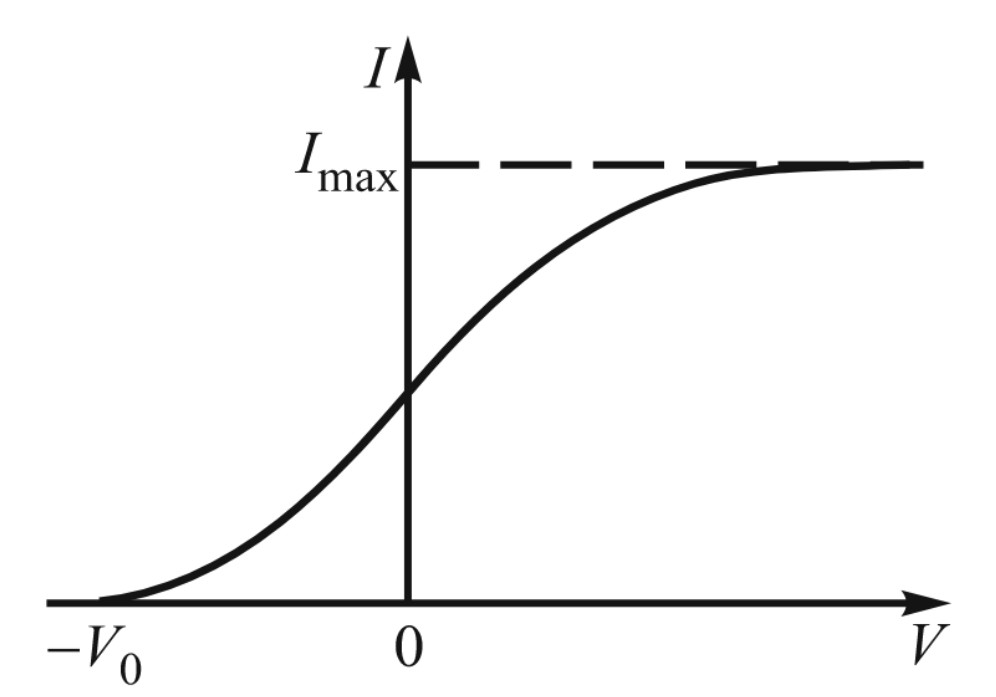
\includegraphics[scale=0.2]{График_1.PNG}
	\end{figure}
	
	При задерживающих потенциалах на анод попадают лишь электроны,  обладающие достаточно большой кинетической энергией,  в то время как медленно движущиеся электроны заворачиваются полем и возвращаются на катод.  При некотором значении $ V = -V_0 $ (потенциал запирания) даже наиболее быстрые фотоэлектроны не могут достичь анода.
	
	Максимальная кинетическая энергия $ E_{max} $ электронов связана с запирающим потенциалом $V_0$ соотношением $ E_{max} = eV_0$.  Получается уравнение Эйнштейна:
	
\[eV_0 = \hbar\omega - W\]
	
	Чтобы определить величину запирающего напряжения,  нам надо правильно экстраполировать получаемую токовую зависимость к нулю,  т. е. определить каковая функциональная зависимость $I(V)$.  Расчет для простейшей геометрии --- плоский катод, освещаемый светом, и параллельный ему анод --- приводит к зависимости:
	
\[\sqrt{I} \propto V_0 - V,\]
	
т. е. корень квадратный из фототока линейно зависит от запирающего напряжения.  
	
	В работе изучается зависимость фототока из фотоэлемента от величины задерживающего потенциала $V$ для различных частот света $\omega$,  лежащих в видимой области спектра. С целью экспериментальной проверки уравнения Эйнштейна определяются потенциалы запирания $V_0$ при разных частотах света и строится зависимость $ V_0(\omega)$,  которая должна иметь вид:
	
\[V_0 (\omega) = \dfrac{\hbar\omega - W}{e}\]
		
	Потенциал запирания $V_0$ для любого катода линейно зависит от частоты света $\omega$.  По наклону прямой на графике $V_0(\omega)$ можно определить постоянную Планка:
	
\[\dfrac{dV_0}{d\omega} = \dfrac{\hbar}{e}\]

	\begin{figure}[h!]
	    \centering
		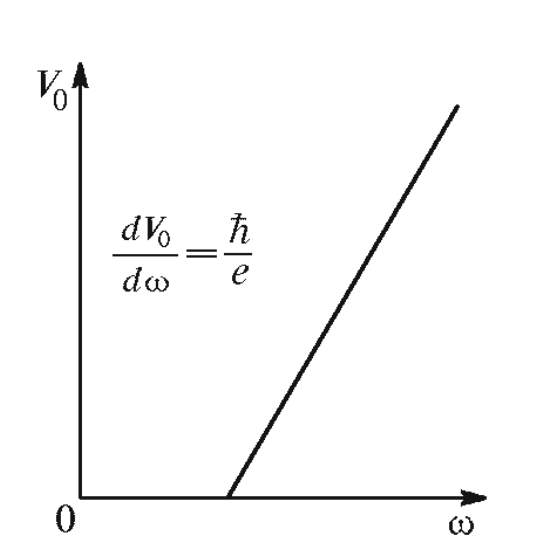
\includegraphics[scale=0.3]{График_2.PNG}
	\end{figure}
	
	Угол наклона прямой $V_0(\omega)$ не зависит от рода вещества,  из которого изготовлен фотокатод.  От рода вещества зависит величина фототока,  работа выхода $W$ и форма кривой $I(V)$.  Все это определяет выбор пригодных для опыта катодов.\\

\newpage
	
\textbf{Экспериментальная установка:}\\\par

	\begin{figure}[h!]
	    \centering
		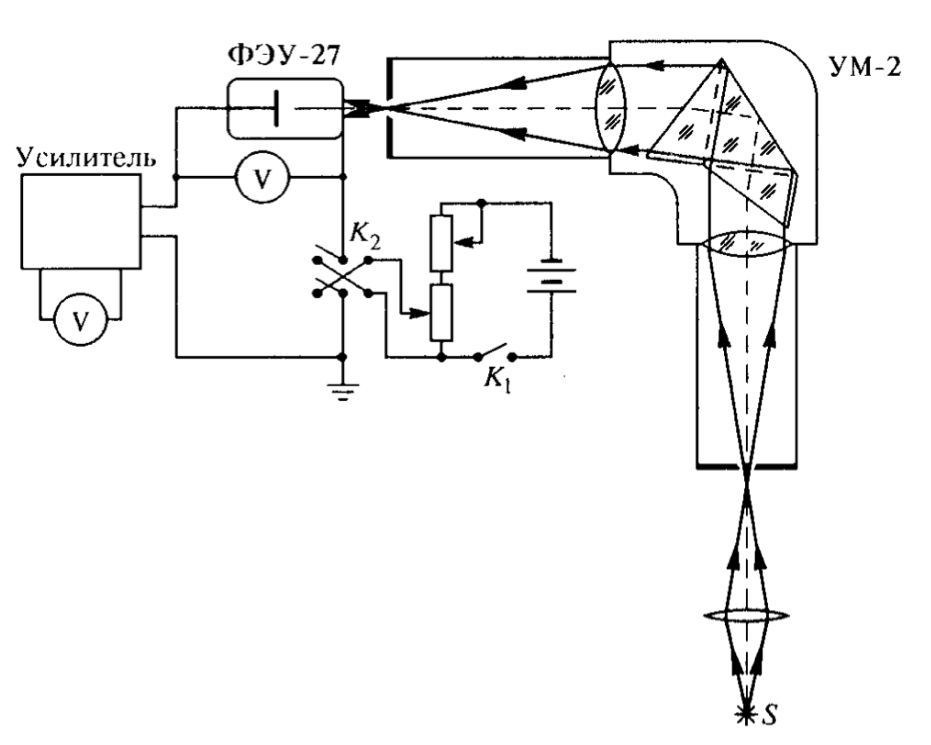
\includegraphics[scale=0.7]{Схема.PNG}
	\end{figure}

	Свет от источника $S$ с помощью конденсатора фокусируется на входную щель призменного монохроматора УМ-2,  выделяющего узкий спектральный интервал,  и попадает на катод фотоэлемента ФЭ.\\
	
\textbf{Ход работы:}\\\par

\begin{enumerate}

	\item Настроим установку.
	
	\item Проведем градуировку барабана по спектру неоновой лампы,  то есть снимем зависимость $\lambda$ от $\theta$:

\newpage
	
	\begin{figure}[h!]
	    \centering
		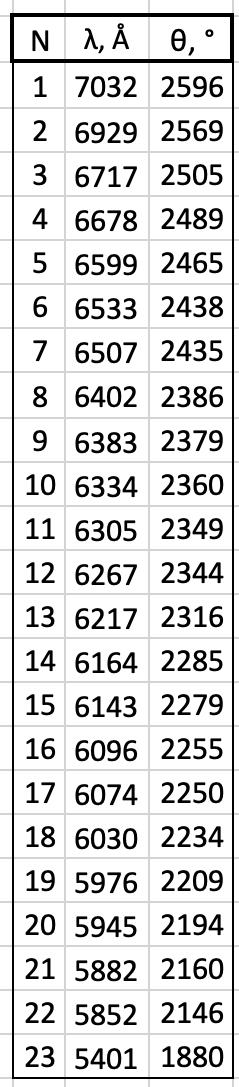
\includegraphics[scale=0.6]{Таблица_1.PNG}
	\end{figure}
	
Построим график:

	\begin{figure}[h!]
	    \centering
		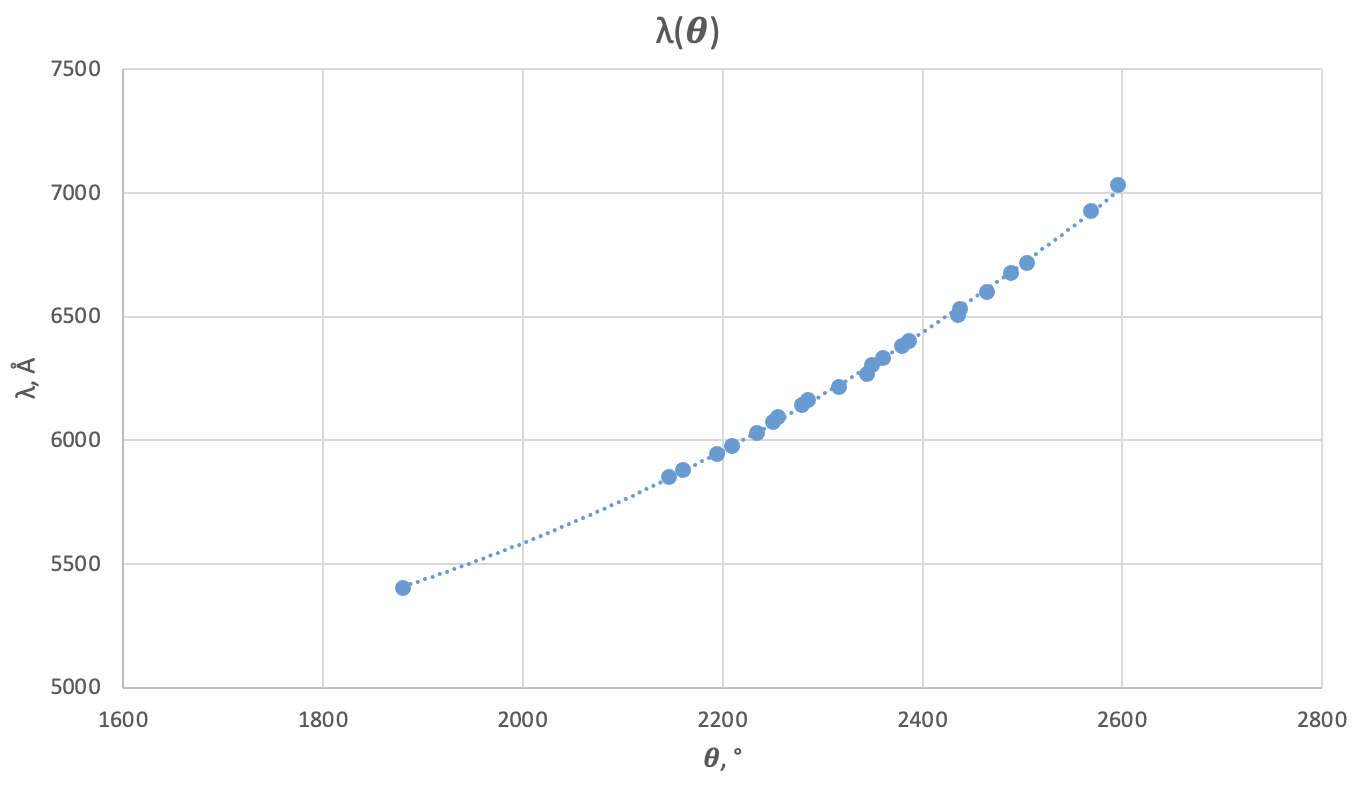
\includegraphics[scale=0.6]{График_3.PNG}
	\end{figure}

	\item Снимем зависимости фототока от напряжения для 6 значений длин 
волн в интервале 540-700 нм (выставляя соответствующие значения,  полученные при градуировке).

	\newpage

	\begin{figure}[h!]
	    \centering
		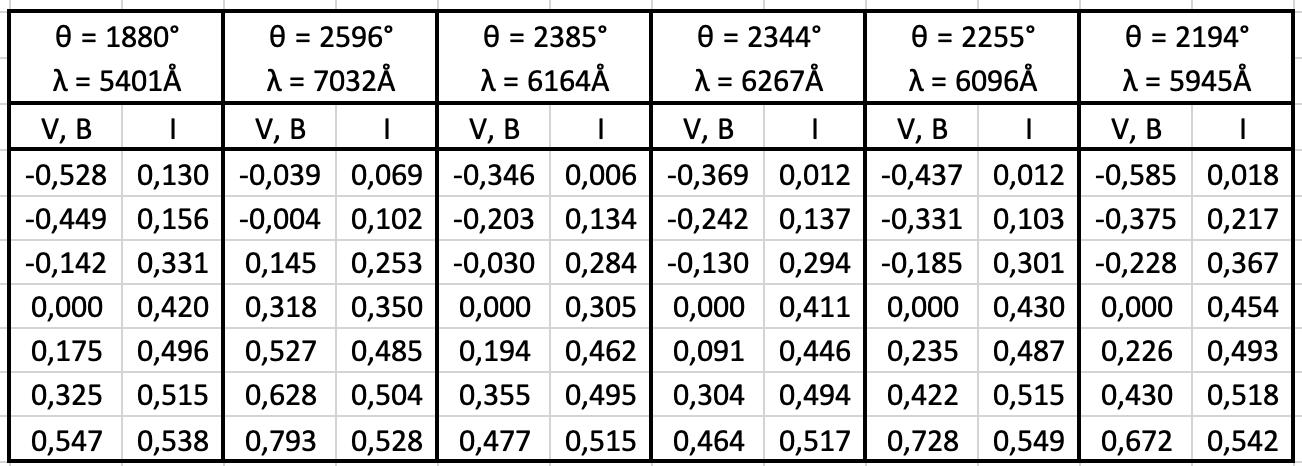
\includegraphics[scale=0.6]{Таблица_2.PNG}
	\end{figure}

	Построим серию графиков $\sqrt{I} = f(v)$.  Для каждой длины волны определим величину запирающего потенциала,  экстраполируя полученные прямые к оси абсцисс. 

	\begin{figure}[h!]
	    \centering
		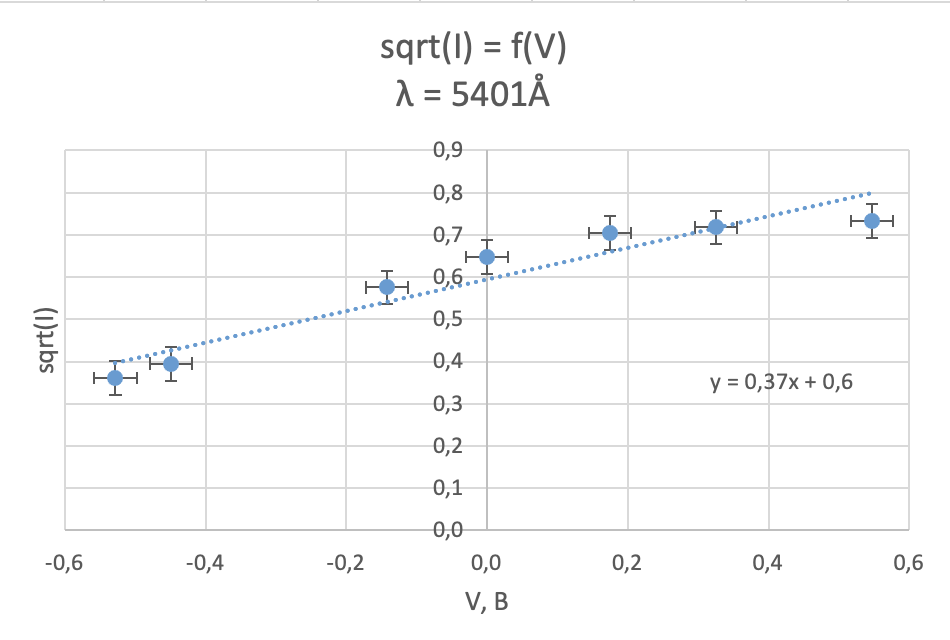
\includegraphics[scale=0.6]{График_4.PNG}
	\end{figure}
	
	\begin{figure}[h!]
	    \centering
		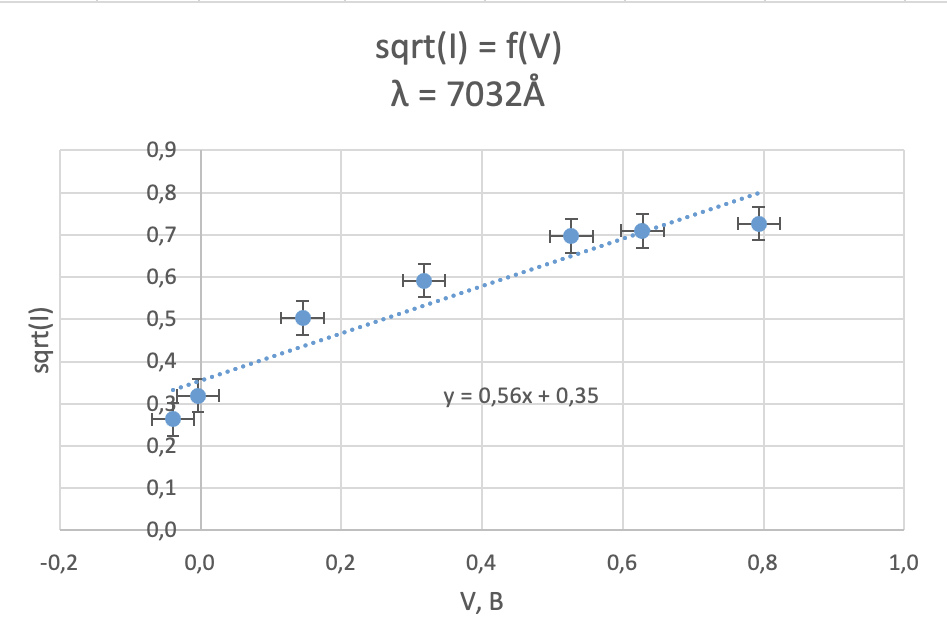
\includegraphics[scale=0.6]{График_5.PNG}
	\end{figure}

	\newpage

	\begin{figure}[h!]
	    \centering
		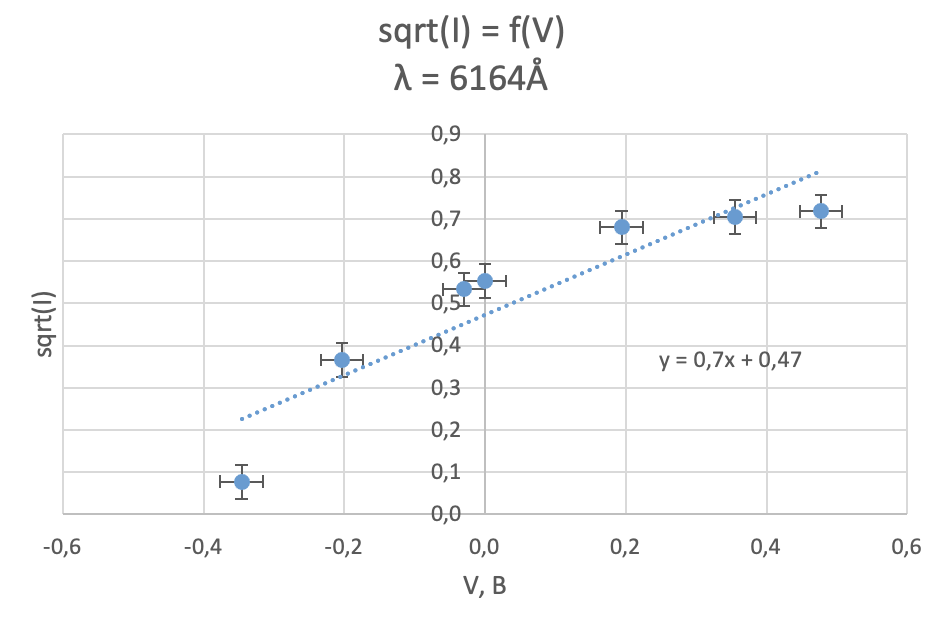
\includegraphics[scale=0.6]{График_6.PNG}
	\end{figure}

	\begin{figure}[h!]
	    \centering
		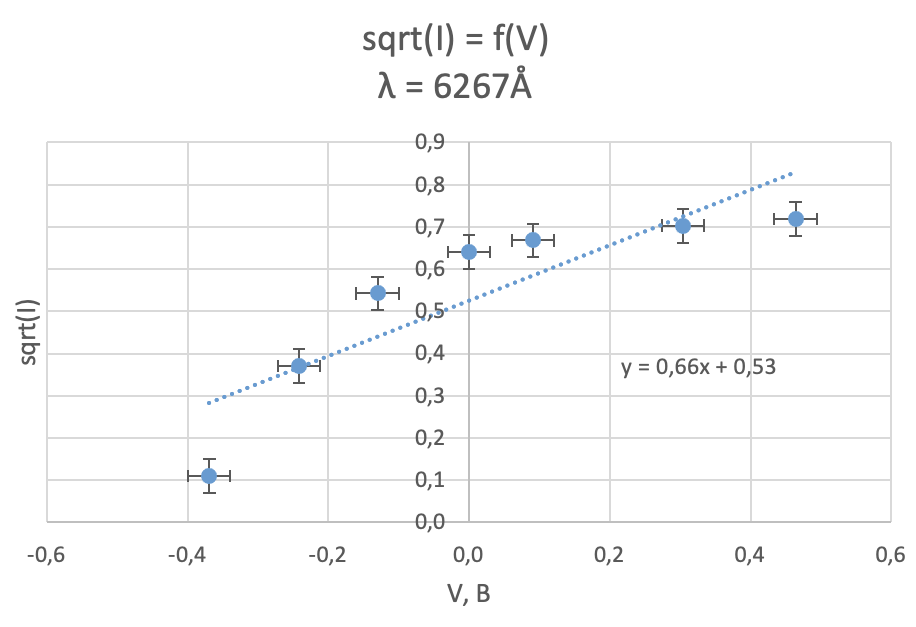
\includegraphics[scale=0.6]{График_7.PNG}
	\end{figure}

	\begin{figure}[h!]
	    \centering
		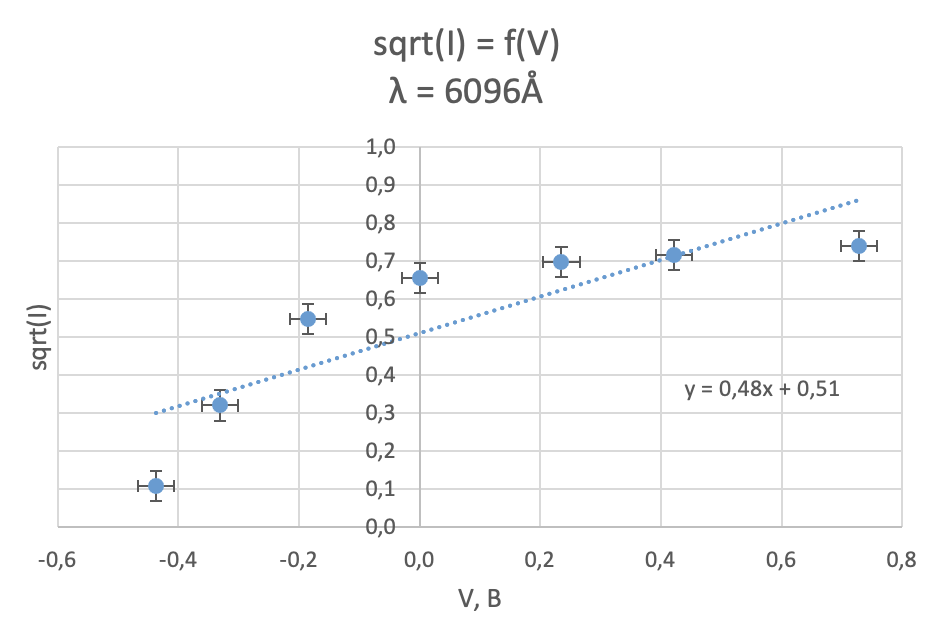
\includegraphics[scale=0.6]{График_8.PNG}
	\end{figure}

	\newpage

	\begin{figure}[h!]
	    \centering
		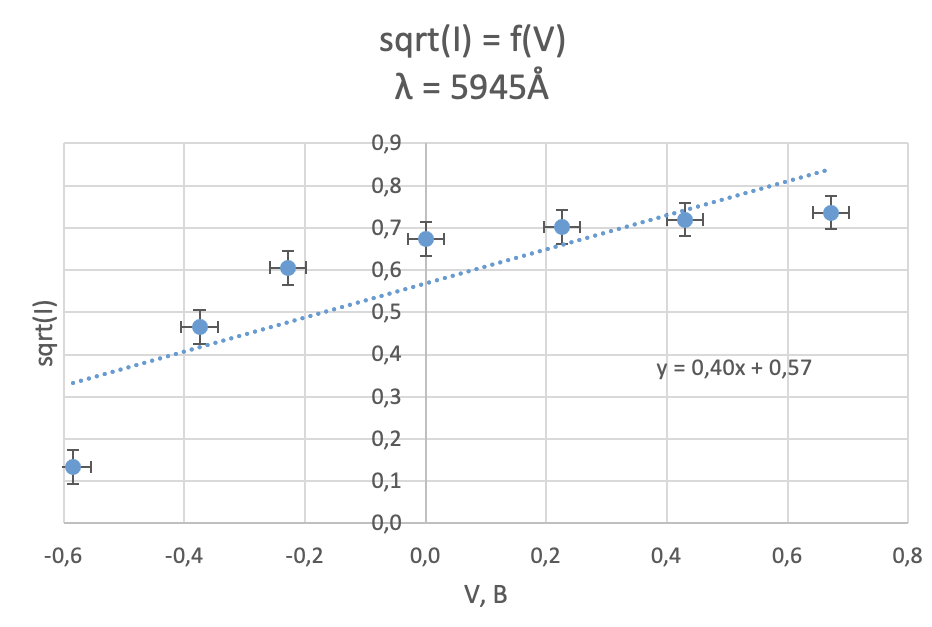
\includegraphics[scale=0.6]{График_9.PNG}
	\end{figure}

	\begin{figure}[h!]
	    \centering
		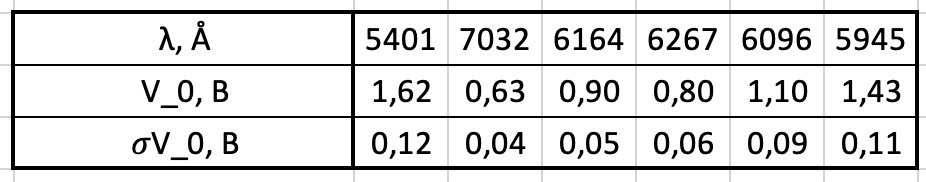
\includegraphics[scale=0.6]{Таблица_3.PNG}
	\end{figure}

\item Построим график зависимости $V_0(\omega)$:

	\begin{figure}[h!]
	    \centering
		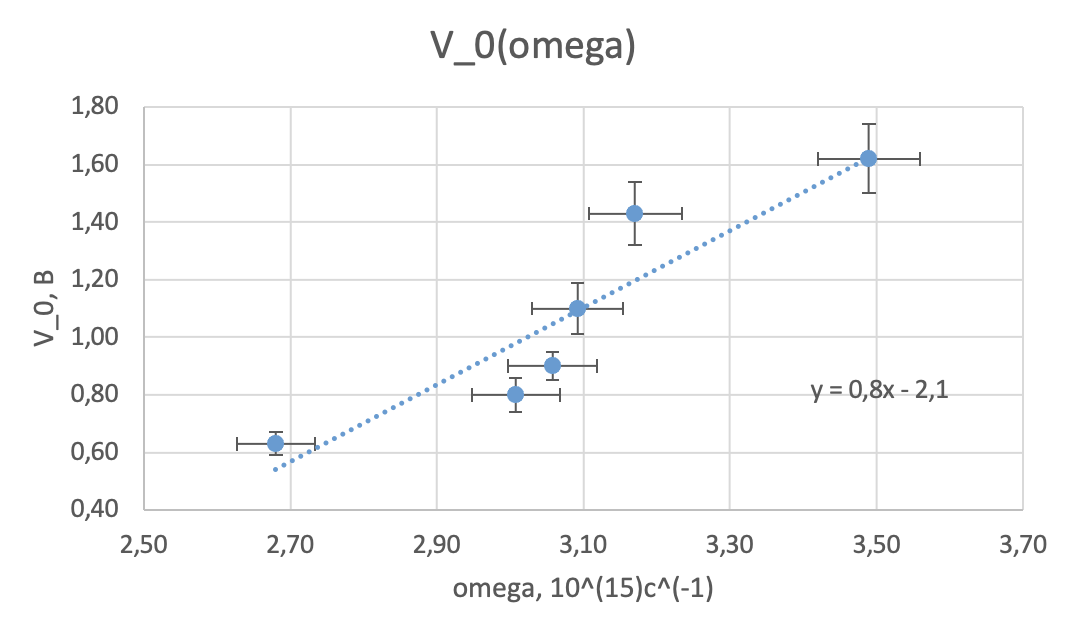
\includegraphics[scale=0.7]{График_10.PNG}
	\end{figure}
	
	Из графика получили значение коэффициента наклона:
	
	\[k = (0,8 \pm 0,1) \cdot 10^{-15} \text{ В} \cdot \text{с}\]
	
	Тогда постоянная Планка:
	
	\[\hbar = (1,28 \pm 0,16) \cdot 10^{-34} \text{ Дж} \cdot \text{с}\]

	 Определим значение красной границы фотоэффекта:
	 
	\[\omega_\text{к} = (2,6 \pm 0,4)\cdot 10^{15} \text{ с}^{-1}\]	 
	 
	Длина волны тогда:
	
	\[\lambda_\text{к} = (7246 \pm 1115) \stackrel{\circ}{A}\] 
	
	Работа выхода:
		 
	\[W = (3,3 \pm 0,5) \text{ эВ}\]	
	  
\end{enumerate}

\textbf{Вывод:}\\\par

В результате выполнения лабораторной работы нами была исследована зависимость фототока от величины задерживающего напряжения: экспериментально проверено,  что квадратный корень из фототока линейно зависит от задерживающего напряжения.

Определена величина постоянной Планка:

\[\hbar_\text{эксп} = (1,28 \pm 0,16) \cdot 10^{-34} \text{ Дж} \cdot \text{с}\]
\[\hbar_\text{теор} = 1,054 \cdot 10^{-34} \text{ Дж} \cdot \text{с}\]

Вычислена красная граница фотоэффекта:

\[\lambda_\text{к} = (7246 \pm 1115) \stackrel{\circ}{A}\] 

И вычислена работа выхода материала катода:

\[W = (3,3 \pm 0,5) \text{ эВ}\]
	
\end{document}